\chapter{Ergebnisse}
In diesem Kapitel werden zunächst
Eigenschaften der Floquet-Theorie an dem Modell überprüft.
Des Weiteren wird die zeitliche Entwicklung
eines Zustandes durch den
Floquet-Formalismus mit der numerischen Lösung der
Schrödingergleichung verglichen. Es wird jeweils ein gemitteleter Strom berechnet und
ebenfalls verglichen.
Zum Ende soll das System auf zwei Elektronen erweitert werden und ebenso ein Strom berechnet werden.
In den folgenden Rechnungen wird der Sprungterm $J=1$ gesetzt und  alle Ergebnisse in Einheiten von J angegeben.
Ebenso gilt dies für alle Naturkonstanten.

\section{Frequenzabbhängigkeit der Quasienergien}
Zu Begin werden die Eigenwerte $\epsilon_{\alpha n}$ für eine Matrix $\mathcal{H}_\mathrm{F}$ mit eine Größe der Matrix $n=1$
bei konstanter lokaler Energie $a=??$ und E-Feldstärke $E_0=??$ für unterschiedliche Frequenz berechnet.
Hier mit soll die Frequenzabhängigkeit \eqref{eqn:epsilon_n} der Eigenwerte der Matrix $\mathcal{H}_\mathrm{F}$
überprüft werden.
Die Eigenwerte $\epsilon_\alpha$ so wie die Eigenwerte $E_{\alpha n}$ des zeitunabhängiges System
die nach der Formel \eqref{eqn:epsilon_n}
sind in der Abbildung \ref{fig:epsilon_f} dargestellt.
\begin{figure}
   \centering
   \includegraphics[width=0.7\textwidth]{C:/Users/daghe/Desktop/Uni/Bachelorarbeit/Freqenzen_kontinuierlich/Plots/Plot_fur_a=2.0_E=0.1.pdf}
   \caption{Eigenwerte $\epsilon_{\alpha n}$ der Matrix $\mathcal{H}_\mathrm{F}$ für $a=??$ und $E_0=??$ in Abhängigkeit von der Frequnez $\omega$.
    Die schwarzen Linien sind die nach der Gleichung \eqref{eqn:epsilon_n} berechneten Eigenwerte für das zeitunabhängige System}
   \label{fig:epsilon_f}
\end{figure}
Aus der Abbildung \ref{fig:epsilon_f} kann entnommen werden, dass die Eigenwerte $\epsilon_{\alpha n}$
(ADD)
\section{Brillouin-Zone der Quasienergien}
Nun sollen versucht werden die Eigenwerte wie in \ref{sec:flotheo} berschrieben in einer Art Brillouin-Zone darzugestellen.
Dafür werden Quasieenergien bei eine konstante Frequenz $\omega=??$ und lokale Energie $a=??$ in Abhängigkeit der
E-Feldamplitude $E_0$,die in einem
Bereich von $0$ bis $0.1 ??$ variiert,  berechnet.
Diese sind in der Abbildung \ref{fig:brillouin} gegen $E_0$ aufgetragen.
Deweiteren wird die Größe $N$ der Matrix $\mathcal{H}_F$ varriert.
% \begin{figure}
%   \includegraphics[width=0.7\textwidth]{C:/Users/daghe/Desktop/Uni/Bachelorarbeit/Energien_kontinuierlich/Plots/Plot_fur_a=2.0_E=0.1.pdf}
%   \caption{}
%     \label{fig:brillouin}
% \end{figure}
Es wird deutlich das zu kleine $N$ die Bedingung für eine Darstellugn in der Brillouin-Zone nicht genügen.
Jedoch für ausreichend großes $N$ können die Quasieenergien $\epsilon_\alpha$ in die erste Brillouin-Zone
mit $-\frac{\omega}{2}<\epsilon_\alpha<\frac{\omega}{2}$ dargestellt werden und
alle anderen Quasieenergien $\epsilon_{\alpha n}$ durch die Periodizitätbedingung \eqref{eqn:epsilon_n} berechnet werden.
Es kann jedoch selbst bei größeren $N$ beobachtet werden, dass bei höheren Zonen?? die Periodizität nicht mehr gegeben ist.

\section{Orthogonalität der Quasizustände}
Im folgendem soll die Orthogonalität zwischen den Quasizuständen $\ket{\Phi_\alpha}$ aus der Gleichung \eqref{eqn:ortho} für
unterschiedliche Größen der Matrix $\mathcal{H}_F$ überpüft werden.
Die Quasiezustände die sich über


-über formel .. kann quasizustand berechnet werden
-die Orthogonalitäts bedingung formel .. sollte erfüllt sein

\section{Zeitentwicklung eines Zustandes durch den Floquet-Formalismus}
-wenn Zustände orthogonal zeitentwicklung möglich
-vergleich mit lsode
-stimmt überein eignet sich folglich für zeitentwicklung

\section{(Strom im System)}
-berechung des Stromes
-überprüfung der quadratischen Ahängigkeit der Stromes
-frequenz abhängigkeit überprüfen (gerade)
-für kleine frequenz problem mit orthogonalität

\section{zwei Elektonen}
